\documentclass{article}

\usepackage{graphicx}
\usepackage{tikz}
\usepackage{tikzsymbols}
\usetikzlibrary{calc,patterns,shapes.geometric}
\pagestyle{empty}
\usepackage[margin=0pt]{geometry}
\geometry{papersize={14in,12in}}

\def\centerarc[#1](#2)(#3:#4:#5){\draw[#1] ($(#2)+({#5*cos(#3)},{#5*sin(#3)})$) arc (#3:#4:#5);}

\begin{document}
	\begin{figure}
		\centering
		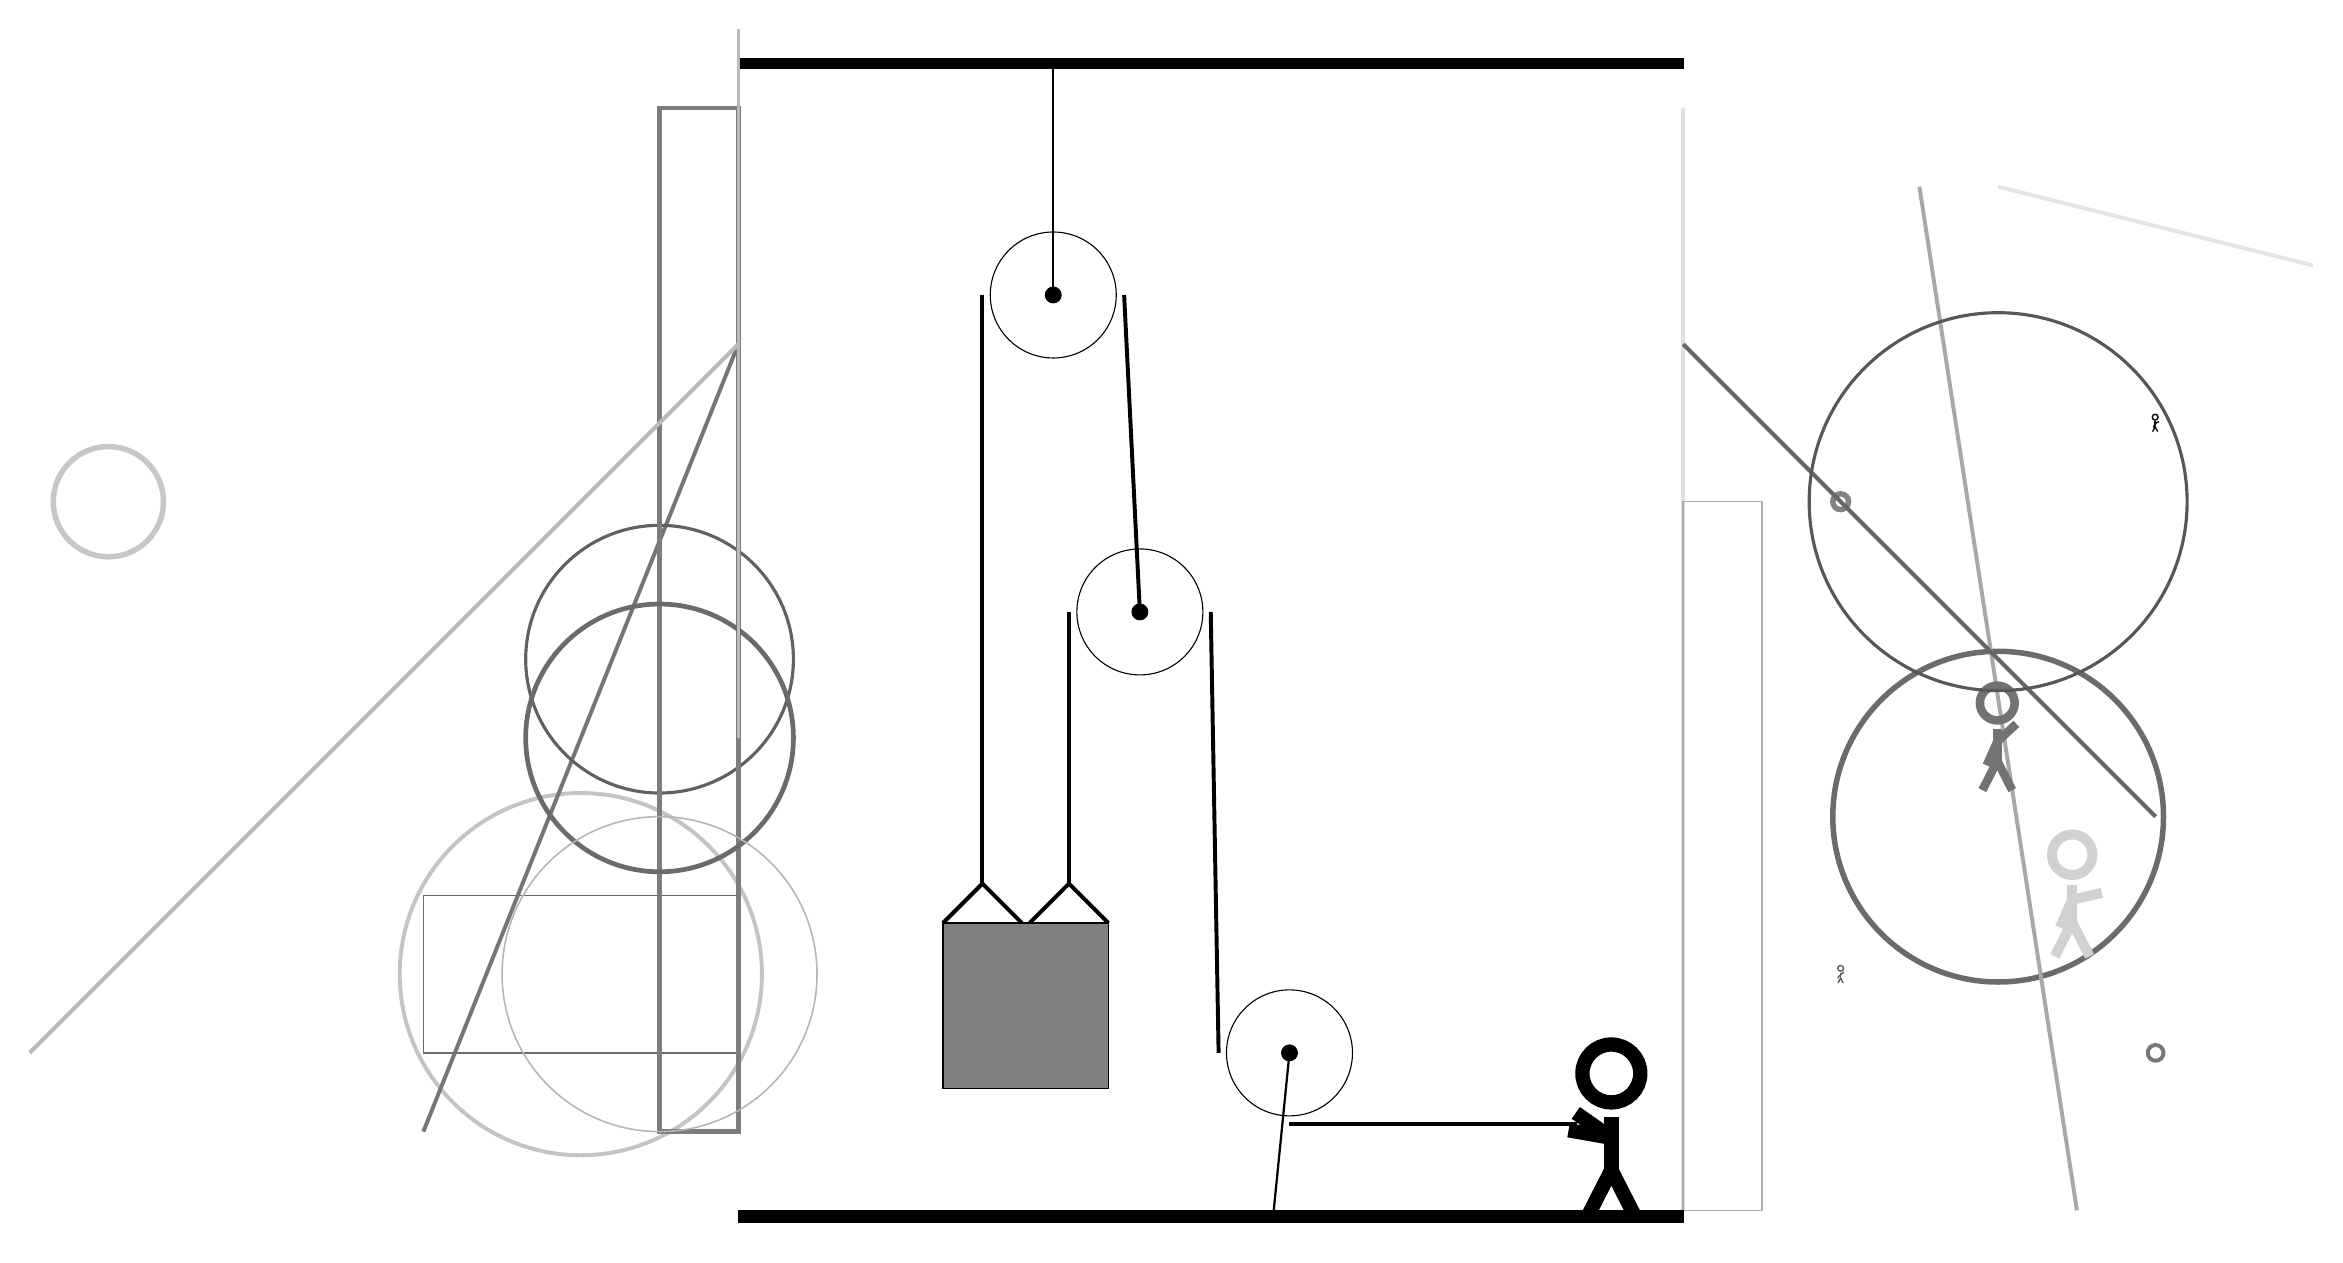
\begin{tikzpicture}
			%%%%% START %%%%%
			
			\draw[fill=black] (-2, 11.5) rectangle (10, 11.625);
			
			\draw (2, 8.625) circle (0.8);
			\draw[fill=black] (2, 8.625) circle (0.1);
			\draw[thick] (2, 8.625) -- (2, 11.5);
			
			\draw (3.1, 4.6) circle (0.8);
			\draw[fill=black] (3.1, 4.6) circle (0.1);
			
			\draw[line width=0.5mm, color=black!12] (10, 11) rectangle (10, -3);
			
			\node[line width=0.4mm, color=black!94] at (16, 7) {\Strichmaxerl[1][66][29]};
			\draw [line width=0.7mm, color=black!58](14, 2) circle (2.1);
			\draw [line width=0.5mm, color=black!23](-4, 0) circle (2.3);
			\draw[line width=0.5mm, color=black!10](14, 10) -- (18, 9);
			\draw[line width=0.5mm, color=black!34](15, -3) -- (13, 10);
			\draw[line width=0.2mm, color=black!59] (-2, -1) rectangle (-6, 1);
			\draw [line width=0.5mm, color=black!53](16, -1) circle (0.1);
			\draw[line width=0.5mm, color=black!54](-6, -2) -- (-2, 8);
			\draw [line width=0.7mm, color=black!49](12, 6) circle (0.1);
			
			\draw [line width=0.4mm, color=black!62](-3, 4) circle (1.7);
			\node[line width=0.7mm, color=black!55] at (14, 3) {\Strichmaxerl[6][66][43]};
			\draw [line width=0.7mm, color=black!64](-8, 8) circle (0.0);
			
			\draw [line width=0.7mm, color=black!22](-10, 6) circle (0.7);
			\draw[line width=0.5mm, color=black!60](10, 8) -- (16, 2);
			\node[line width=0.2mm, color=black!18] at (15, 1) {\Strichmaxerl[7][66][13]};
			
			\draw[line width=0.6mm, color=black!51] (-3, 11) rectangle (-2, -2);
			\draw [line width=0.6mm, color=black!58](-3, 3) circle (1.7);
			\draw[line width=0.4mm, color=black!27] (-2, 12) rectangle (-2, 3);
			\draw [line width=0.2mm, color=black!29](-3, 0) circle (2.0);
			\node[line width=0.7mm, color=black!63] at (12, 0) {\Strichmaxerl[1][44][43]};
			
			\draw[line width=0.5mm, color=black!27](-2, 8) -- (-11, -1);
			
			\draw [line width=0.4mm, color=black!66](14, 6) circle (2.4);
			\draw[line width=0.2mm, color=black!32] (10, 6) rectangle (11, -3);
			
			\draw (5, -1) circle (0.8);
			\draw[fill=black] (5, -1) circle (0.1);
			\draw[thick] (5, -1) -- (4.8, -3);
			
			\draw[line width = 0.5mm]  (0.6, 0.65) -- (1.1, 1.15) -- (1.6, 0.65);
			\draw[line width = 0.5mm]  (1.7, 0.65) -- (2.2, 1.15) -- (2.7, 0.65);
			\draw[fill=black!50] (0.6, 0.65) rectangle (2.7, -1.45);
			
			\draw[line width = 0.5mm] (1.1, 8.625) -- (1.1, 1.15);
			\centerarc[line width = 0.5mm](2, 8.625)(0:180:0.9);
			\draw[line width = 0.5mm] (2.9, 8.625) -- (3.1, 4.6);
			\draw[line width = 0.5mm] (2.2, 4.6) -- (2.2, 1.15);
			\centerarc[line width = 0.5mm](3.1, 4.6)(0:180:0.9);
			\draw[line width = 0.5mm] (4.0, 4.6) -- (4.1, -1);
			\centerarc[line width = 0.5mm](5, -1)(180:270:0.9);
			\draw[line width = 0.5mm] (5, -1.9) -- (8.65, -1.9);
			
			\node at (9, -2) {\Strichmaxerl[10][-35][170]};
			
			\draw[fill=black] (-2, -3) rectangle (10, -3.15);
			
			%%%%% END %%%%%
		\end{tikzpicture}
	\end{figure}	
\end{document}